%-----------------------------------------------------------------------------%
\addChapter{Lampiran A 1}
\chapter*{Lampiran A}
%-----------------------------------------------------------------------------%

\begin{figure}
    \begin{center}
        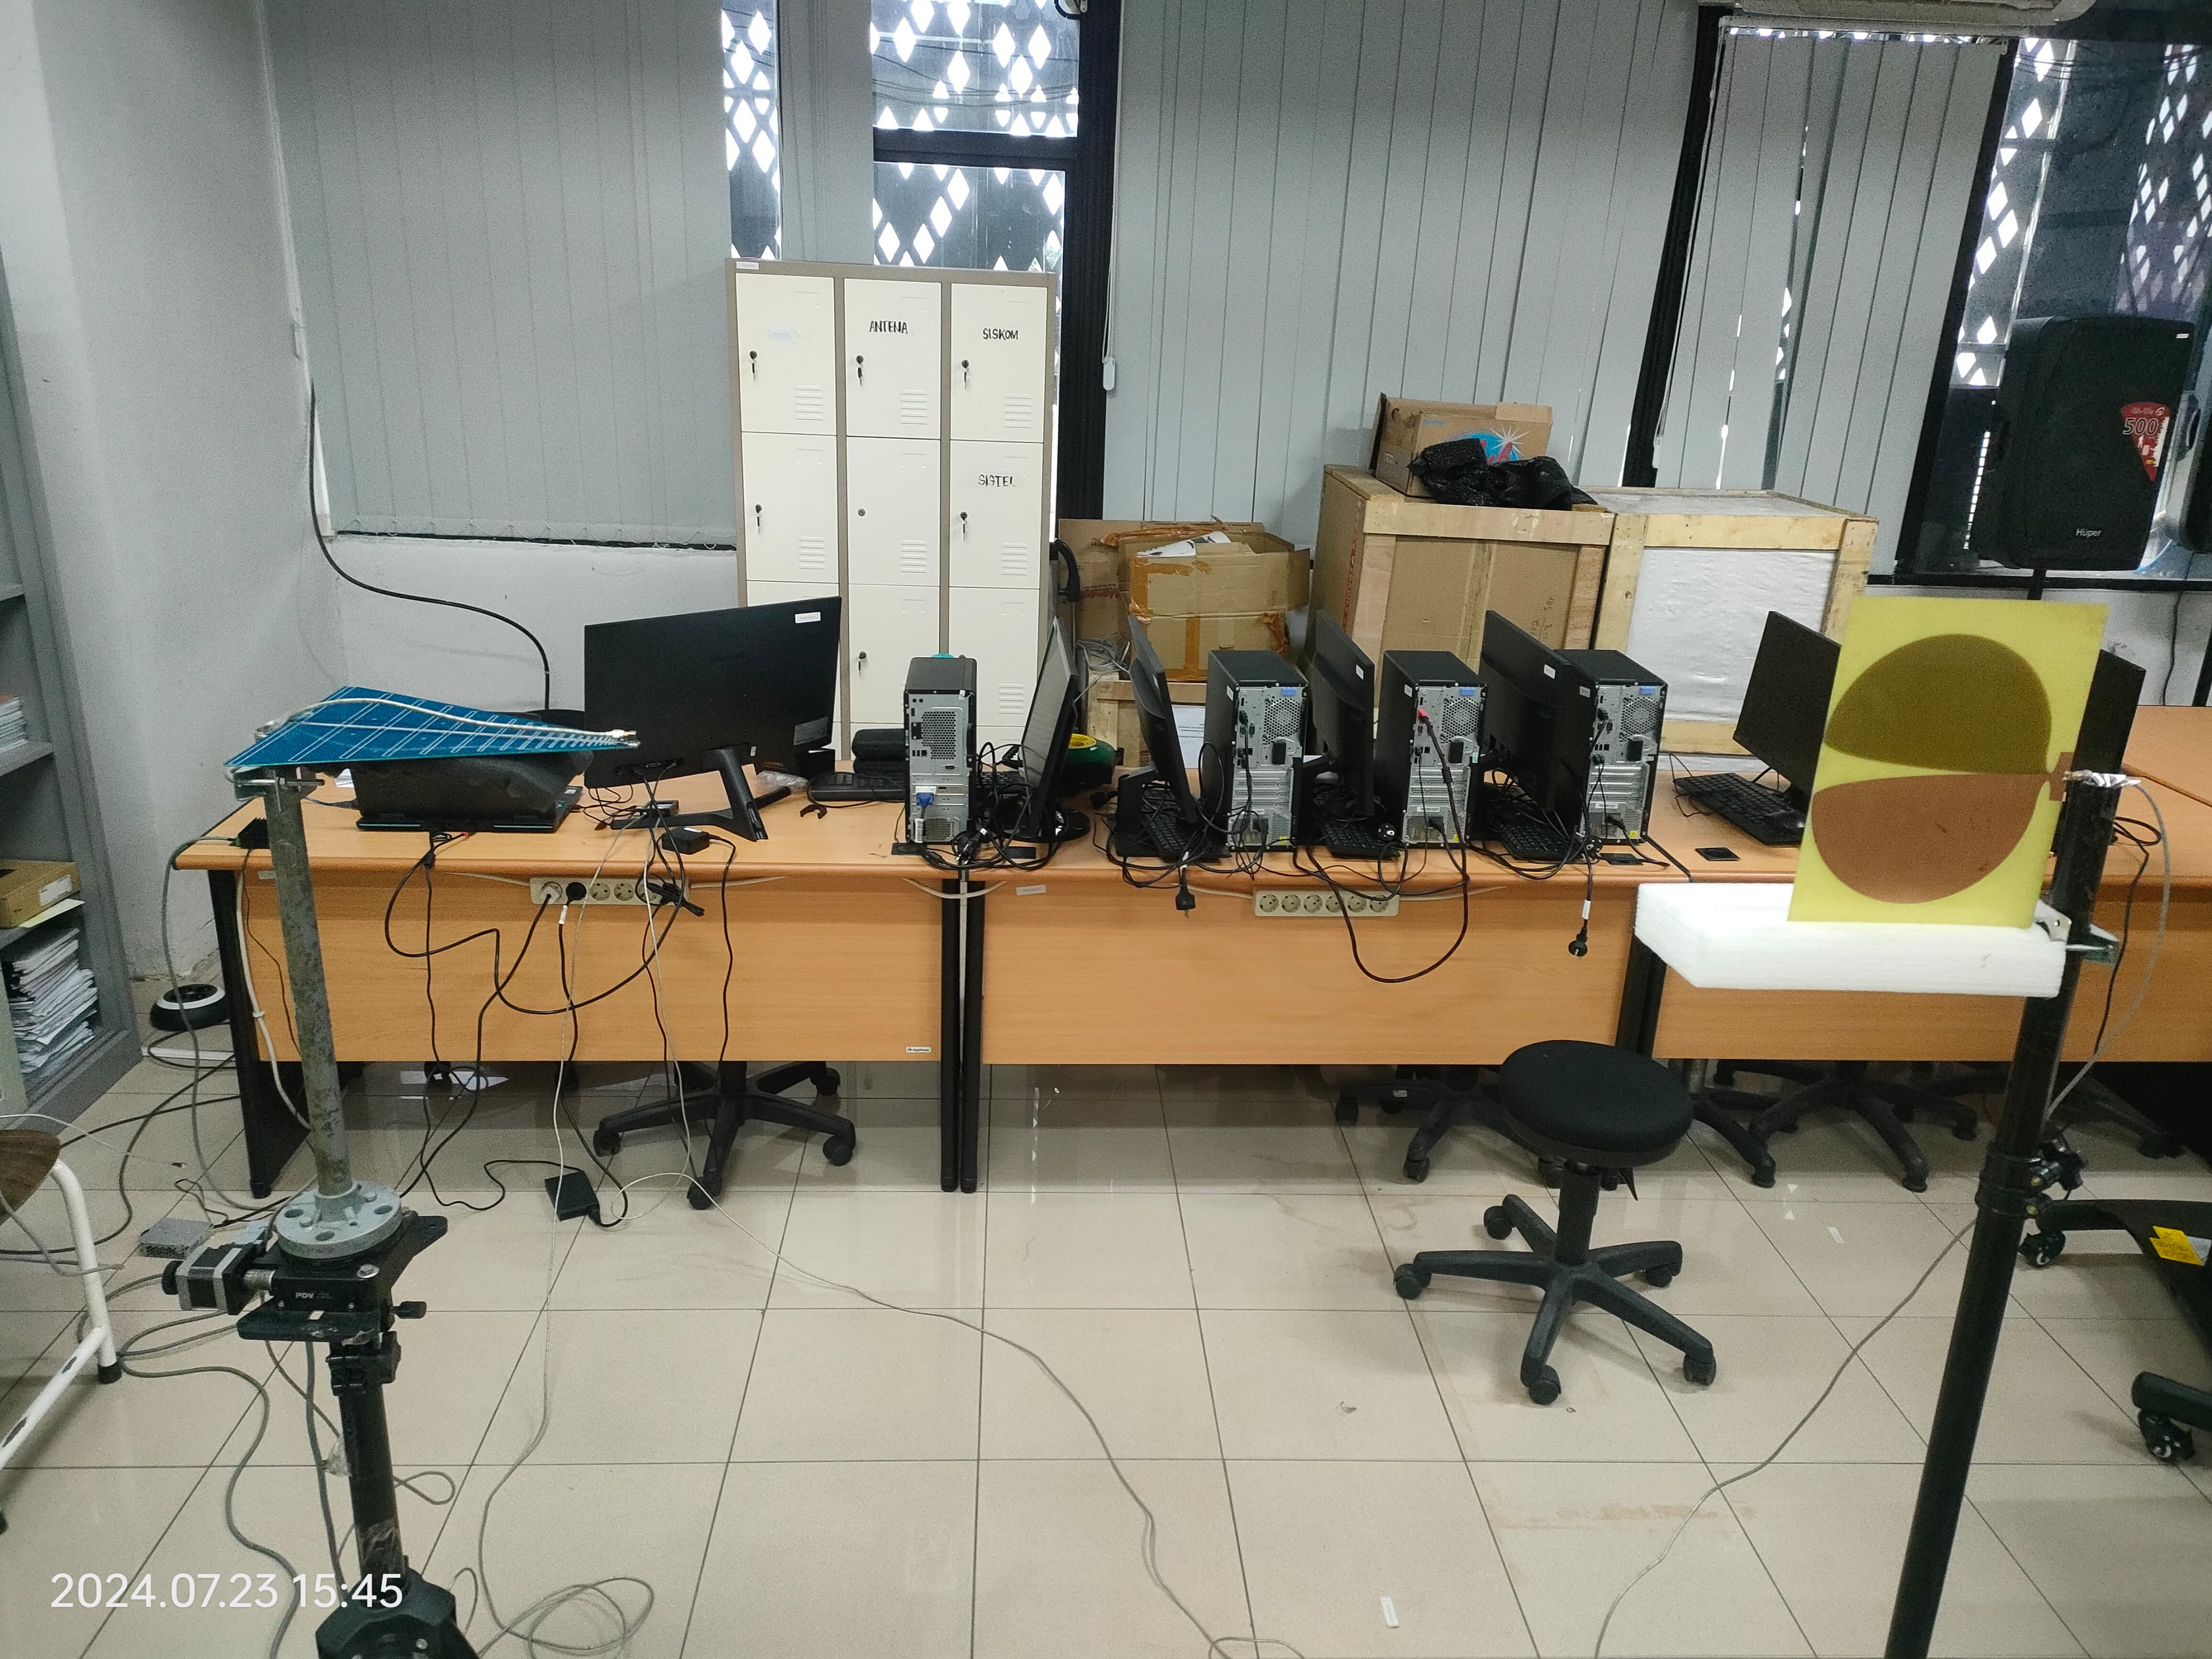
\includegraphics[scale=0.08]{pics/Lampiran/Horizonal.jpg}
    \end{center}
\end{figure}

\addChapter{Lampiran A 2}
\begin{figure}
    \begin{center}
        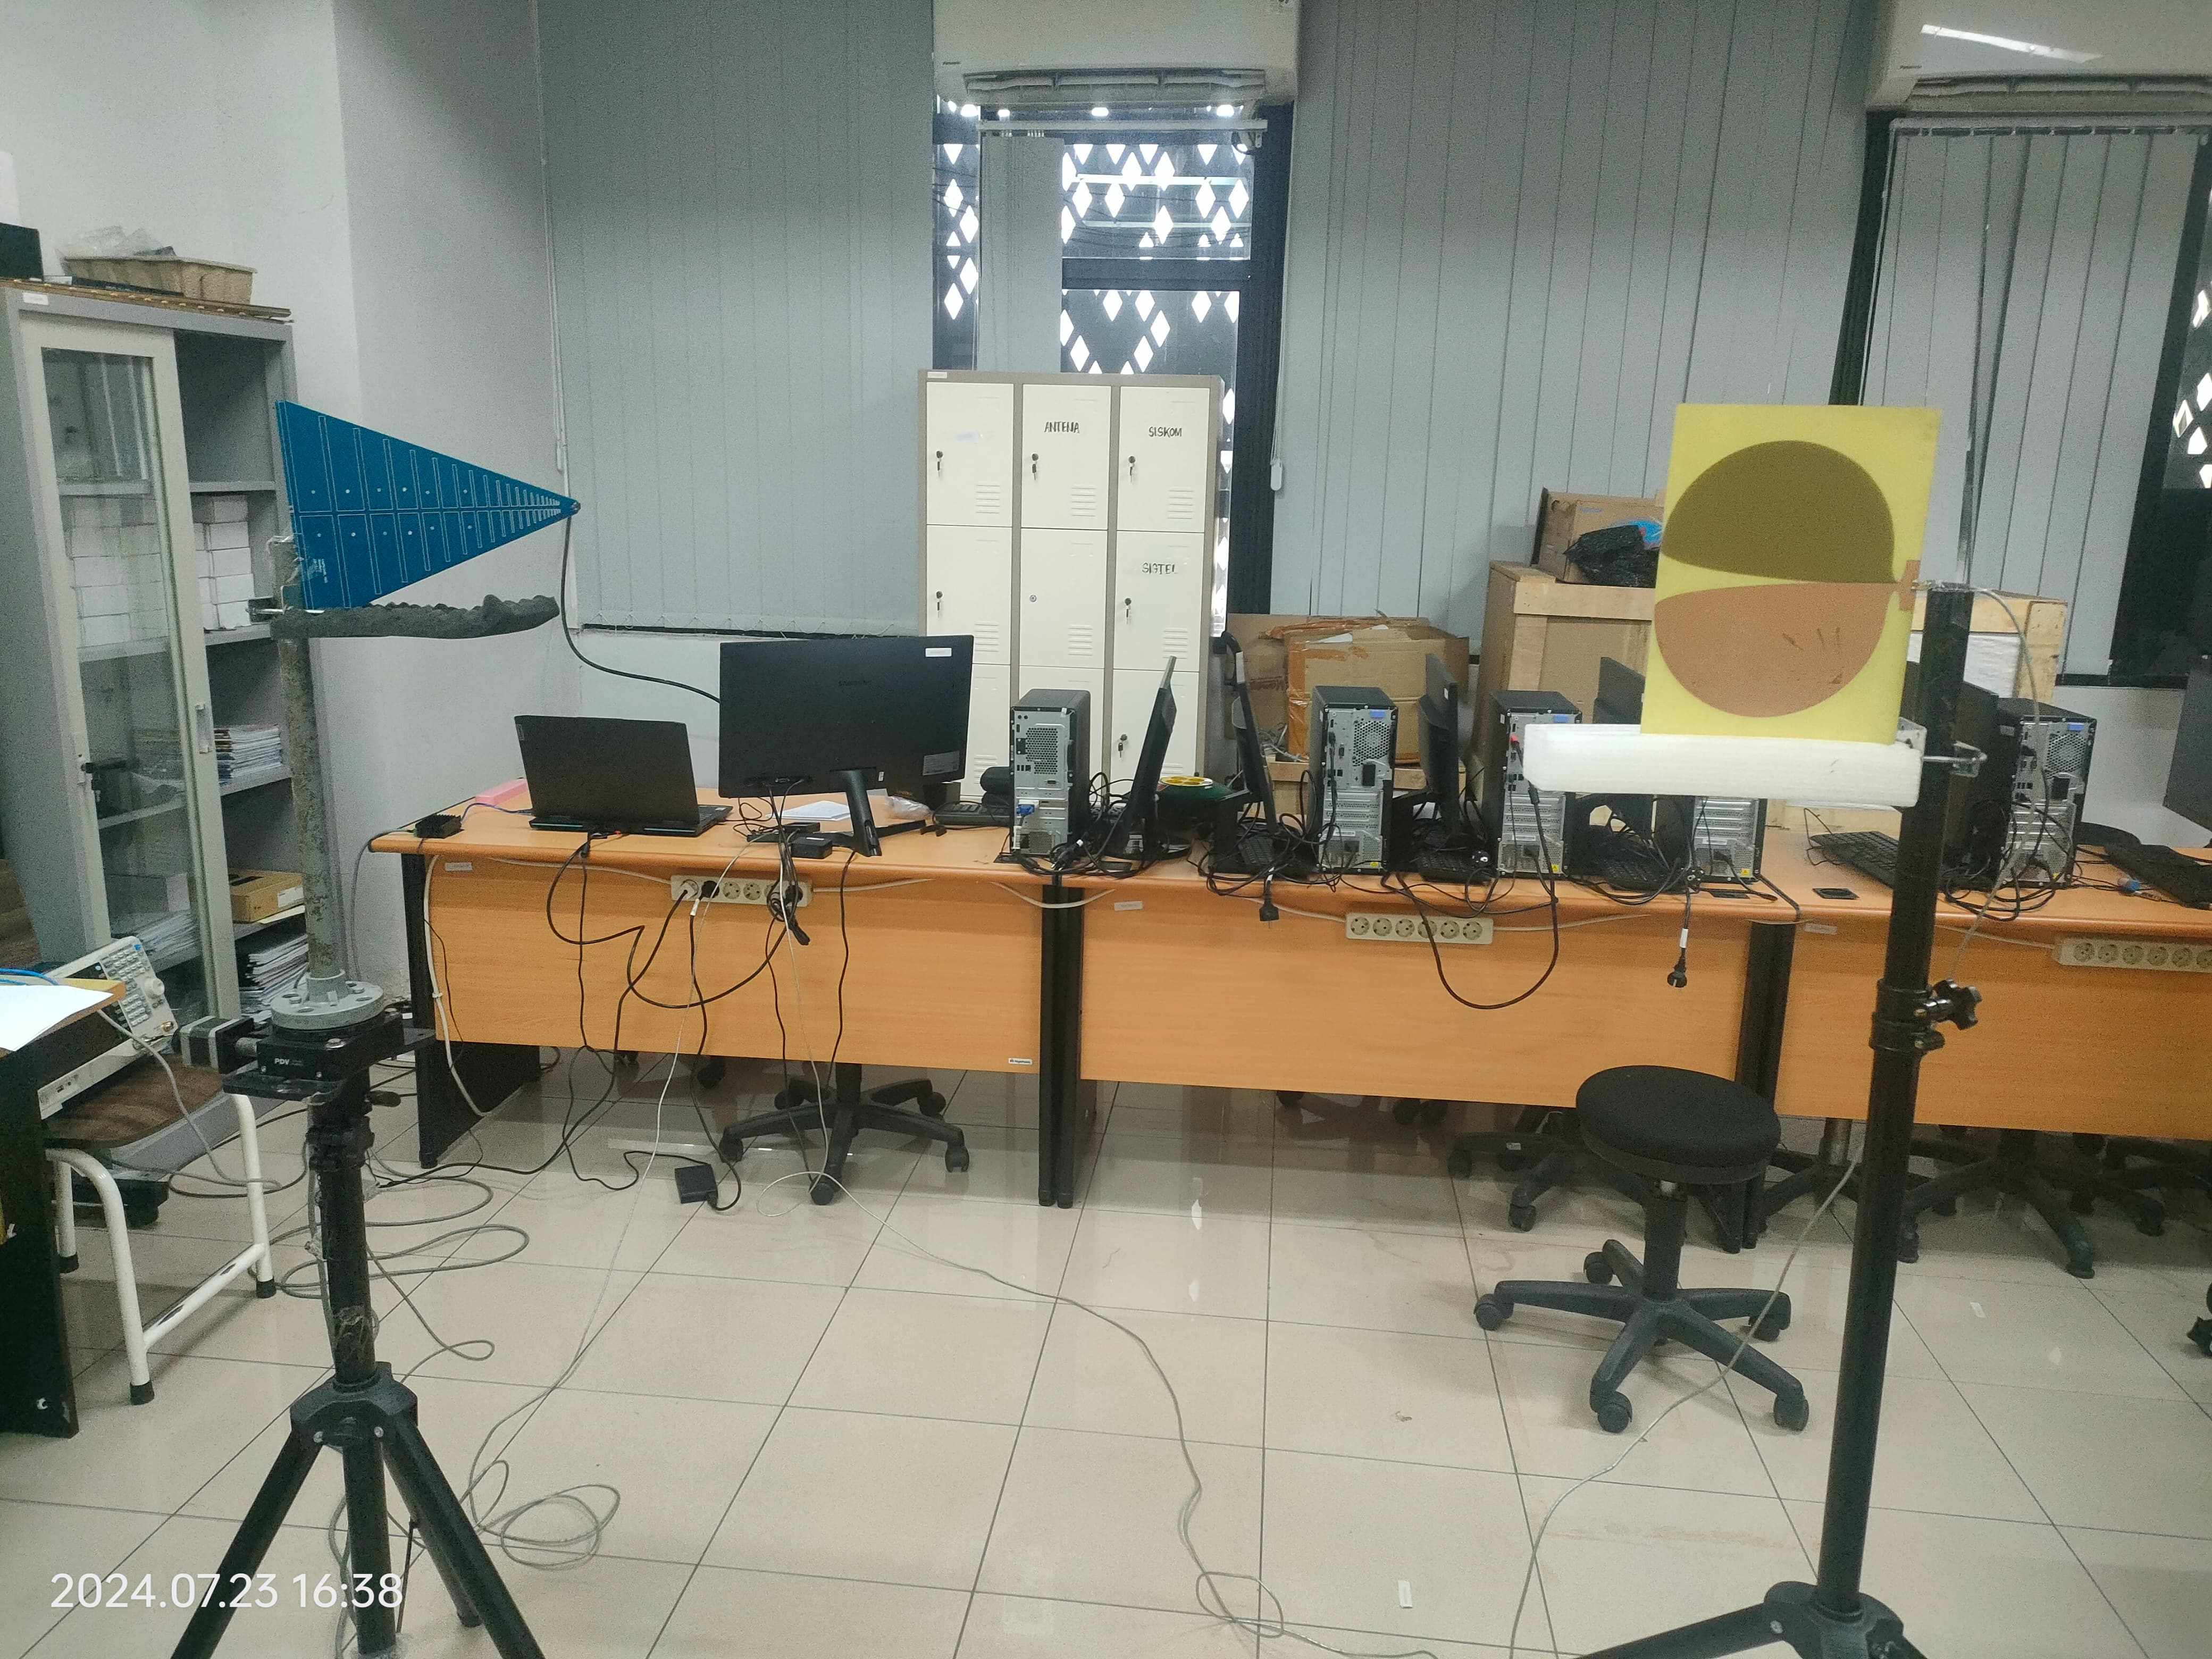
\includegraphics[scale=0.08]{pics/Lampiran/Vertikal.jpg}
    \end{center}
\end{figure}

%-----------------------------------------------------------------------------%
\addChapter{Lampiran B}
\chapter*{Lampiran B}
%-----------------------------------------------------------------------------%

\lstinputlisting[language=Matlab]{pics/Lampiran/ReadTransmitSignal.m}

%-----------------------------------------------------------------------------%
\addChapter{Lampiran C}
\chapter*{Lampiran C}
%-----------------------------------------------------------------------------%

\lstinputlisting[language=Matlab]{pics/Lampiran/postProcessingRange.m}